\documentclass{article}
\usepackage{graphicx}
\usepackage{caption}
\usepackage{subfig}
\usepackage{hyperref}
\usepackage{amsmath}
\begin{document}
Robotic SLAM 
\section{Introduction}
Terms 

\begin{itemize}
    \item State estimation - find out the pose 
    \item Localisation - pose w.r.to landmark or map
    \item Mapping 
   \item navigation and motion planning - a star, wave front dijkstra 
\end{itemize}

\subsection{What is SLAM}
    Computing robot's poses and the map of the environment at the 
    same time.
\textbf{Localisation} : estimating robots location\\ 
\textbf{Mapping}      : building a MAP\\

\textbf{Given}

\begin{itemize}
    \item Robots control inputs   $$u_{1:T} = \{u_1,u_2,u_3....u_T\}$$
    \item Observations $$z_{1:T} = \{z_1,z_2,z_3,...,z_T\}$$
\end{itemize}

\textbf{Wanted}
\begin{itemize}
    \item Map of the environment $$m$$
    \item path of the Robot $$x_{0:T} = \{x_0,x_1,x_2,...,x_T\}$$
\end{itemize}

Using the robots control inputs we can predict the position of the robot.
From the observations $z_{1:T}$, we can calculate the position of the robot. 
Both the steps have some error associcated with it . Lets call the first
one the model noise and second one the sensor noise. So we have to associate 
a probability with both of them. The error accumulates over time(even if the
error in individual measurements is really small)\\

So in the probalistic terms our problem minimises to 
$$p(x_{0:T},m|z_{1:T},u_{1:T})$$


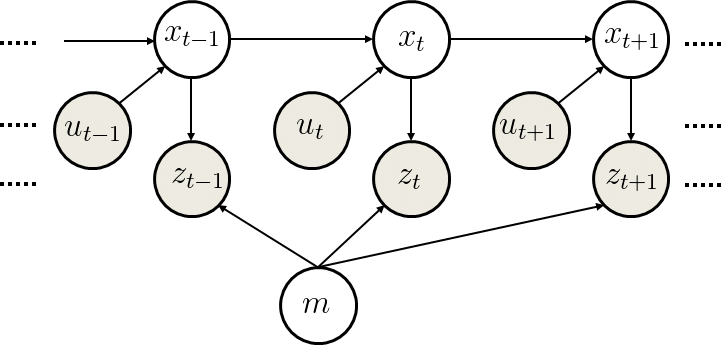
\includegraphics[width = \linewidth]{graphical_model.png}
\subsection{Full Slam vs online SLAM}
    \begin{itemize}
        \item Full SLAM estimates the entire path $$p(x_{0:T},m|z_{1:T},u_{1:T})$$
        \item Online SLAM estimates only the most recent pose $$p(x_{t},m|z_{1:T},u_{1:T})$$
    \end{itemize}
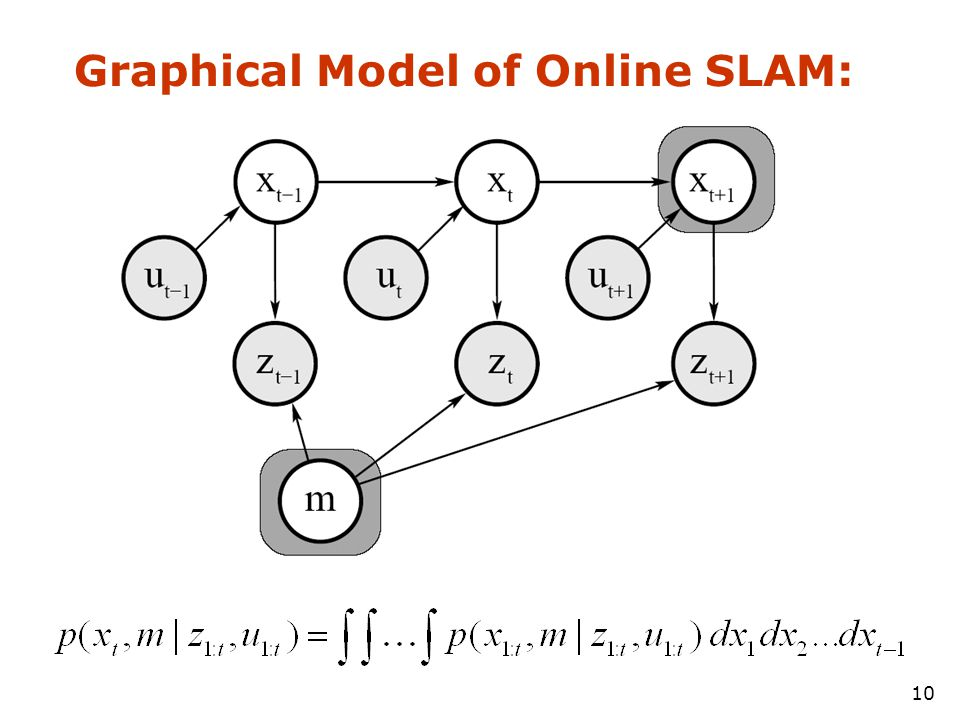
\includegraphics[width = \linewidth]{online_SLAM.jpg}

\subsection{Types of SLAM}
    occupancy maps created from lidars, sonars etc. - volumetric SLAM
    feature based approach - store features and localise based on that 
    volumetric SLAM maybe  better for navigation applications . 
    Topological representations vs geometric representations.
    Static vs dynamic features.
    Active - robot decides the path so as to build a map vs passive slam -
    may follow a fixed path i.e. path not optimised for mapping/ exploration
\section{Bayes Filter}
\subsection{State Estimation}
    \textbf{Goal} $p(x|z,u)$
    \newline
    \textbf{Recursive Bayes Filter} 

\begin{align*}  
    bel(x_t) & = p(x_t | z_{1:t},u_{1:t})\\
    & = \eta p(z_t|x_t,z_{1:t-1},u_{1:t}) * p(x_t | z_{1:t-1},u{1:t})\\
    & = \eta p(z_t|x_t) * p(x_t | z_{1:t-1},u{1:t})\\
    & = \eta p(z_t|x_t) \int_{x_{t-1}} p(x_t |x_{t-1}, z_{1:t-1},u_{1:t}) * p(x_{t-1}|z_{1:t-1}u_{1:t-1})dx_{t-1}\\
    & = \eta p(z_t|x_t) \int_{x_{t-1}} p(x_t |x_{t-1},u_t) * bel(x_{t-1})dx_{t-1}
 \end{align*}
 we can split this into predict and update steps where\\
 \textbf{Predict Step} 
 $$\overline{bel(x_t)} =  \int_{x_{t-1}} p(x_t |x_{t-1},u_t) * bel(x_{t-1})dx_{t-1}$$
 \textbf{Update Step} 
 $$bel(x_t) =  \eta * p(z_t | x_t) * \overline{bel(x_t)}$$


 \textbf{Bayes filter} gives a framework for recursive state estimation using
 the above equations. The actual realisation  may be kalman filtering , EKF or
 particle filter
 (Linear\ non linear motion models )
 (distributions)
 \textit{Kalman Filter} -  Gaussians , requires linear or linearised model 
 \textit{Particle filter} - Non-parametric , Arbitrary models
 
 \subsection{Probability motion models}
 $p(x_t | u_t,x_{t-1})$ we can model this in two ways 
 \begin{itemize}
     \item odometry models - measurement of velocity (tends to be more accurate)
     \item velocity models - we know the input commands, but no measurement of vel
 \end{itemize}
 \subsection{Model for laser scanners}
 scan z consisits of k beams $z_t \,\epsilon \, \Re^{k}$ i.e. 
 $z_t = \{z_t^1,z_t^2,.....z_t^k\}$,\\ Assuming 
 beams are independednt, then $$p(z_t|x_t,m) = \prod_{i = 1}^{k} p(z_t^i|x_t,m)$$
 \begin{itemize}
     \item Beam endpoint model (likelihood calculated as gaussian blur on occupancy map)
     \item Ray cast model (occlusion, sensor accuray, satuaration , random)
     \item model for range bearing sensors $z_t^i  = (r_t^i,\phi_t^i)^T$
        $$r_t^i = ||m-x|| + gaussian$$
        $$\phi_t^i = \angle (m-x) - \theta + gaussian$$


 \end{itemize}

\section{Kalman filter Equations}
\begin{align*}
    \bar{\mu_t} & = g(u_t,\mu_{t-1})\\
    \bar{\Sigma_t} & = G_t \Sigma_{t-1} G_t^T + R_t\\
    K_t & = \bar{\Sigma_t}H_t^T(H_t\bar{\Sigma_t}H_t^T + Q_t)^{-1}\\
    \mu_t & = \bar{\mu_t} + K_t(z_t - h(\bar{\mu_t}))\\
    \Sigma_t & = (I - K_tH_t)\bar{\Sigma_t}
\end{align*}
\subsection{Summary}
\begin{itemize}
    \item Diverge for large non linearities 
    \item Can deal only single modes 
    \item Successful in medium scale scenes with good data associations
    \item Approximations exists to reduce the computational complexity
\end{itemize}
\textbf{commonly used Datasets:}
\begin{itemize}
    \item Victoria Park Data sets - Trees are the landmark -Data assosciation -girth and height
    \item Tennis Court Dataset - for mapping precescion
\end{itemize}
\section{Extended Kalman Filter vs Unscented Kalman Filter}
\textbf{EKF} works by linearising the state transfer equations 
thus making sure that all the conditional and marginal distributions 
will remain gaussian. Gaussians are closed space. \textbf{UKF} uses
the nonlinear state transmission equation, then tries to sample a 
gaussian distribution from the non-gaussian resulted from the non-linear
operation. 
\subsection{Strategy for chosing sampling points and weights for UKF}
\begin{align*}
X^{[0]} &= \mu\\
X^{[i]} &= \mu + (\sqrt{(n+\lambda)\Sigma})_i  \; for\: i = 1,...,n\\
X^{[i]} &= \mu - (\sqrt{(n+\lambda)\Sigma})_i  \; for\: i = n+1,...,2n\\
w_m^{[0]} &= \frac{\lambda}{n + \lambda}\\
w_c^{[0]} &= w_m^{[0]} + (a -\alpha^2 + \beta)\\
w_m^{[i]} = w_c^{[i]} &= \frac{1}{2(n+\lambda)} \: for \: i = 1,....,2n
\end{align*}
where $\alpha \, \epsilon \, (0,1]$; $k>= 0$ ; $\lambda = \alpha^2(n+k) - n$;\\
too small value of K will lead to UKF ~ EKF . Too large - diverge\\
$\sqrt{\Sigma} =  VD^{1/2}V^{-1}$ , we are sampling the gaussian along the eigen vectors
of the covariance matrix. \\
$$\bar\mu_t = \sum_{1 = 0}^{2n}w^{[i]}g(X^{[i]})$$
$$\bar\Sigma_t = \sum_{1 = 0}^{2n}w^{[i]}(g(X^{[i]}) - \bar\mu_t)(g(X^{[i]}) - \bar\mu_t)^T + R_t$$
\section{Grid Maps}

SLAM problems can make one of the types of maps
\begin{itemize}
    \item \textbf{Feature Based Maps:} Maps is repsented by a few lanndmarks. Advantage of this type of maps is the space time complexity can be smaller compared to Volumetric Maps. On the downside, we have to implement a feature detector - i.e. observations are not directly used in this method. 
        \begin{figure}
            
            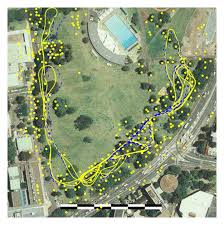
\includegraphics[width = \linewidth]{./feature_maps.jpeg}
            \caption{Feature map imposed over victoria park}
        \end{figure}

\item \textbf{Volumetric Maps:} Volumetric Maps on the other hand uses all observations and represent the map using a 3D(lidar point cloud) or 2D(range sensor) grid. Occupancy is often shown with a black pixel and free areas are white. Unseen areas are marked with grey. Feature based maps are used in kalman filter implementations, Particle filter based approaches use Grid mapping  
    \begin{figure}%
    \centering
    \subfloat[3D grid map from lidar point cloud]{{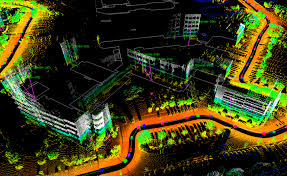
\includegraphics[width=0.32\linewidth]{./3dGrid.jpeg} }}%
    \qquad
    \subfloat[Occupancy Grid Map]{{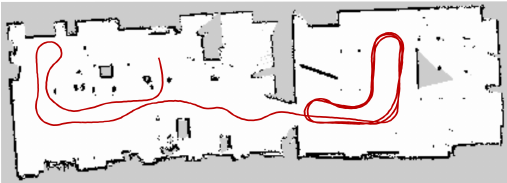
\includegraphics[width=0.6\linewidth]{./gridMap.png} }}%
    \caption{Volumetric Maps}%
    \label{fig:example}%
    \end{figure}
\end{itemize}

\section{Links and references}

Webpage from Syrill Stachniss can be found \href{http://ais.informatik.uni-freiburg.de/teaching/ws13/mapping/}{here}\\
\href{https://pythonrobotics.readthedocs.io}{pythonrobotics}
\end{document}

